\capitulo{2}{Introducción}


%Descripción del contenido del trabajo y de la estructura de la memoria y del resto de materiales entregados.


\section{Conceptos teóricos básicos.}

%Explicación de los conceptos teóricos básicos necesarios para que cualquier miembro del tribunal pueda entender el trabajo realizado.

%Esta sección puede contener el número de subsecciones que sean necesarias.

\subsection{Sistema muscular}

El sistema muscular es el responsable de generar los movimientos del cuerpo, ya sean voluntarios e involuntarios. Esto es fundamental para mantener la postura corporal, generar calor, estabilizar las articulaciones y para el correcto funcionamiento de los órganos vitales como el corazón. 
El tejido muscular se puede clasificar en tres tipos: esquelético, cardíaco y liso \cite{alma991000263829705771}.

\begin{itemize}
    \item \textbf{Músculo liso}: se encuentra principalmente en las paredes de los órganos viscerales huecos como el estómago o la vejiga urinaria. Las células son unicelulares, con forma de huso, por lo que no son estriadas y no se controla de forma voluntaria.
    \item \textbf{Músculo cardíaco}: se localiza únicamente en el corazón y mueve la sangre a través del aparato circulatorio. Al igual que el músculo esquelético, sus fibras son estriadas y no está controlado de forma voluntaria como el músculo liso. Las fibras musculares cardíacas son células ramificadas con un solo núcleo que se unen mediante discos intercalados y están protegidas por tejido conectivo blando. 
    \item \textbf{Musculo esquelético}: músculo estriado que se encuentra adherido al esqueleto permitiendo controlar el movimiento corporal. Cada músculo esquelético está formado por un conjunto de fibras largas y cilíndricas protegidas por tejido conectivo y controladas por neuronas motoras somáticas, con lo cual, no pueden iniciar su propio movimiento de contracción.

    Una fibra muscular se compone  del sarcolema, que es la membrana celular y en su interior se encuentra el sarcoplasma. Está formada por miofibrillas que son cadenas de pequeñas unidades contráctiles denominadas sarcómeros. Dentro de cada uno, se encuentran los filamentos gruesos (miosina) y filamentos finos (actina). Además, incluye el retículo sarcoplasmático y túbulos T (Figura \ref{fig:fibra-muscular}).

    % IMAGEN FIBRA MUSCULAR
    \begin{figure}[ht]
    \centering
    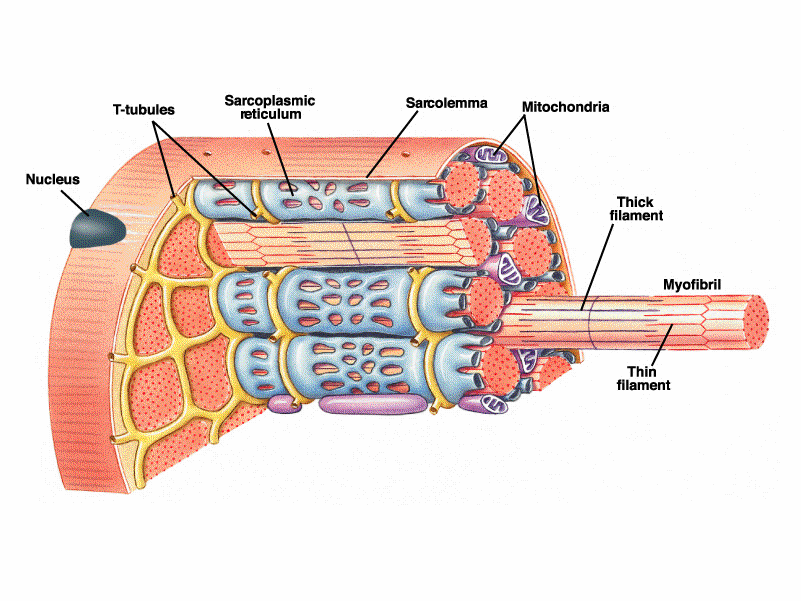
\includegraphics[width=0.7\textwidth]{img/fibra-muscular.png}
    \caption{Estructura anatómica de una fibra muscular esquelética \cite{website:docplayer}.}
    \label{fig:fibra-muscular}
    \end{figure}

\end{itemize}


El sistema nervioso controla los movimientos produciendo un efecto en los músculos. Los movimientos se pueden clasificar en tres categorías:

\begin{enumerate}
    \item \textbf{Movimientos reflejos}: son integrados principalmente en la médula espinal. Además, el tronco encefálico y el cerebelo controlan los reflejos posturales, los cuales ayudan a mantener la posición del cuerpo, los ojos y las manos.
    \item \textbf{Movimientos voluntarios}: son responsabilidad de la corteza cerebral y de los ganglios basales. Pueden ser iniciados a voluntad y aquellos que son aprendidos pueden convertirse en movimientos involuntarios.
    \item \textbf{Movimientos rítmicos}: son una combinación de movimientos voluntarios y reflejos como el acto de caminar. Se inician y terminan por aferencias de la corteza cerebral y los generadores de patrones centrales (redes de inteneuronas del SNC \footnote{Sistema Nervioso Central: constituido por el cerebro y la médula espinal y controlan todas las funciones del cuerpo}) mantienen los movimientos una vez activados.
\end{enumerate}


La mayoría de las señales enviadas para producir el movimiento voluntario son transmitidas desde la corteza a la medula espinal a través del tracto corticoespinal. Igualmente, las señales de los ganglios basales viajan por las vías extrapiramidales para influir en el movimiento corporal.



\subsection{Ganglios basales}

Los \textbf{ganglios basales (GB)} son núcleos subcorticales interconectados constituidos por el núcleo estriado (caudado y putamen), el globo pálido interno (Gpi) y externo (Gpe), la sustancia negra pars compacta (SNpc) y sustancia negra pars reticulada (SNr), el núcleo subtalámico (NST) y el núcleo ventro-lateral del tálamo, como se puede observar en la figura \ref{fig:ganglios-basales}. Son los encargados de controlar el movimiento a través de dos vías, directa e indirecta \cite{MARTINEZFERNANDEZ2016363}. Además, las neuronas de los ganglios basales presentan múltiples sinapsis en el SNC constituyendo el tracto o sistema extrapiramidal \cite{alma991000263829705771}.

% IMAGEN GANGLIOS BASALES
 
\begin{figure}[ht]
    \centering
    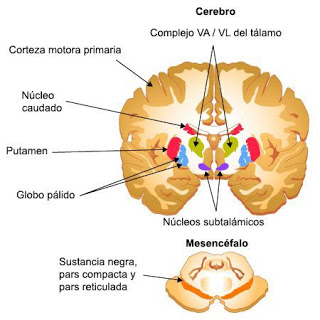
\includegraphics[width=0.4\textwidth]{img/ganglios-basales.jpg}
    \caption{Estructura anatómica de los ganglios basales: núcleo estriado, globo pálido, sustancia negra, núcleos subtalámicos y núcleo ventro-lateral del tálamo \cite{website:Síndesi}.}
    \label{fig:ganglios-basales}
\end{figure}

El núcleo estriado contiene neuronas espinosas de tamaño mediano (NEMs) de naturaleza GABAérgica e interneuronas colinérgicas\footnote{Neuronas que emplean la acetilcolina (ACh) como neurotransmisor.} y GABAérgica que emplean GABA (ácido gama amino butírico), un neurotransmisor inhibidor. Las NEMs de la vía directa expresan receptores dopaminérgicos D1 que facilitan el movimiento, mientras que en la vía indirecta predominan los receptores dopaminérgicos D2 que lo inhiben \cite{avila2014ganglios}. El funcionamiento de ambas vías se muestran en la figura \ref{fig:ganglios-vias} .

Por una parte, la vía directa normalmente está excitada por la liberación de dopamina sobre los receptores de dopamina D1, los cuales liberan una mayor cantidad de GABA. Como consecuencia, la actividad del globo pálido interno se ve disminuida y libera menos GABA, lo que estimula al tálamo. Éste libera glutamato y excita la corteza motora.  Cuando disminuye los niveles de dopamina, las neuronas se inhiben, lo que inactiva el complejo Gpi/SNr y el tálamo envia menos impulsos excitatorios a la corteza motora que se manifiesta en forma de temblor.

Por otra parte, la vía indirecta está inhibida por la liberación de dopamina en los receptores D2. El globo pálido externo está estimulado y libera GABA. El núcleo subtalámico está inhibido y libera menor cantidad de glutamato, lo que se traduce en una disminución de la actividad del globo pálido externo, así como una menor producción de GABA. El tálamo es excitado y libera glutamato para estimular la corteza  motora. La deficiencia de dopamina en EP, hace que las neuronas inhiban el globo pálido externo y, éste a su vez activa el núcleo subtalámico. De forma que, el complejo Gpi/SNr se activa y la actividad del tálamo se inhibe impidiendo la generación del movimiento, dando lugar a la bradicinesia \cite{marin2018enfermedad}.

% IMAGEN VIA DIRECTA E INDIRECTA

\begin{figure}[ht]
    \centering
    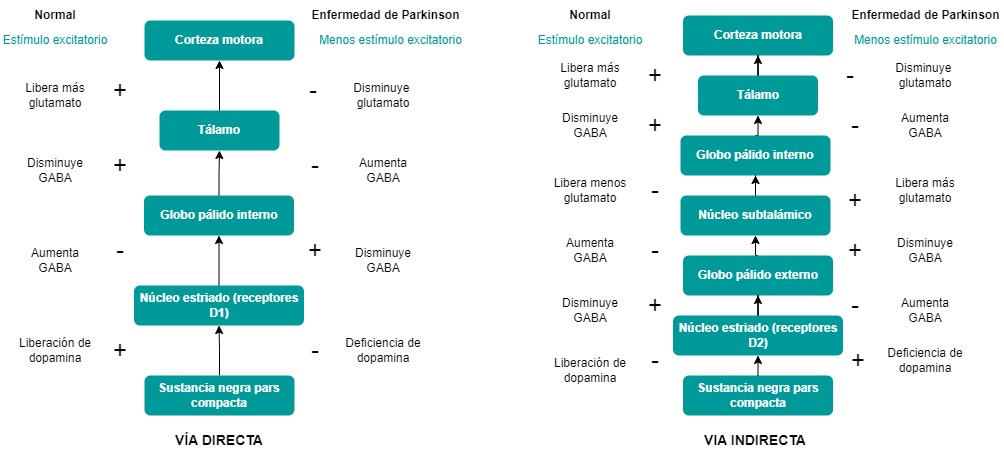
\includegraphics[width=1\textwidth]{img/Diagrama_ganglios.jpg}
    \caption{Vías directa e indirecta y su alteración en la enfermedad de Parkinson \cite{marin2018enfermedad}.}
    \label{fig:ganglios-vias}
\end{figure}


\subsection{Enfermedad de Párkinson}

La \textbf{enfermedad de Parkinson (EP)} es un trastorno neurodegenerativo que afecta de manera crónica y progresiva al sistema nervioso central. Es la segunda enfermedad neurodegenerativa más frecuente después del Alzehimer y los síntomas, así como la evolución de la enfermedad varían de unos individuos a otros \cite{MARTINEZFERNANDEZ2016363}.  

Se caracteriza por la pérdida o degeneración de neuronas dopaminérgicas localizadas en la parte compacta de la sustancia negra (SNpc) que forma parte de los ganglios basales y liberan dopamina, así como la presencia de cuerpos de Lewy siendo depósitos de proteína alfa-sinucleína que se acumulan dentro de las neuronas \cite{ayala2007enfermedad, gomez2012mecanismos, MARTINEZFERNANDEZ2016363}.  

 Esta afectación de los ganglios basales conlleva una disminución de los valores de dopamina, una sustancia que transmite la información necesaria para la realización del movimiento. De forma que, los receptores dopaminérgicos no son estimulados correctamente y, como consecuencia, causa alteraciones en el control del movimiento y mantenimiento de la postura corporal \cite{ayala2007enfermedad}.

 En España, hay al menos 300.000 habitantes que padecen EP y un nuevo caso por 10.000 habitantes al año \cite{GARCIARAMOS2016401}. Varios estudios han demostrado que tanto la prevalencia como la incidencia de la enfermedad de Parkinson es mayor en hombres que en mujeres \cite{MARTINEZFERNANDEZ2016363}.


\subsubsection{Etiología}

En la actualidad se desconoce la causa de dicha enfermedad. Sin embargo, puede deberse a una combinación de factores genéticos, medioambientales y los derivados del propio envejecimiento del organismo \cite{ayala2007enfermedad, MARTINEZFERNANDEZ2016363}. 

\begin{itemize}
    \item Edad: se trata de un factor de riesgo. Suele iniciarse entre los 50-80 años. Aproximadamente un 1\% de la población mayor de 60 años padece dicha enfermedad.
    \item Factores genéticos: una mutación genética específica suele ser el origen en el caso de la EP de inicio joven ( menores de 40) y se asocia a una herencia autosómica recesiva. En el 50\% de los casos familiares y en el 15\% de los esporádicos, la mutación más común es la del gen de la parkina.
    \item Factores medioambientales: según algunos estudios, el consumo de agua de pozo o la exposición a pesticidas y herbicidas pueden ser factores de riesgo.
\end{itemize}


\subsubsection{Manifestación clínica}
Cada individuo puede presentar distintos síntomas y evolucionar de forma diferente. Los pacientes con EP se caracterizan por presentar manifestaciones motoras asimétricas, ya que las alteraciones predominarán más en un lado del cuerpo que en el otro.\cite{neri2017sintomas}.

\begin{itemize}
    \item \textbf{Temblor en reposo}: es el síntoma más característico y está presente en el 70\% de los casos. No obstante, la falta de de temblor en reposo no excluye el diagnóstico, ya que puede estar ausente en el 30\% de los pacientes. Afecta frecuentemente a las manos, la cara, los pies, la mandíbula y los músculos de la lengua. Asimismo, algunos pacientes pueden presentar temblor postural que se manifiesta al adoptar una postura.
    \item \textbf{Bradicinesia}: hace referencia a la lentitud de movimientos. Incluye la hipocinesia, que es la reducción de la amplitud del movimiento y la acinesia, la dificultad para el movimiento. A medida que la enfermedad progresa, el paciente presenta mayor dificultad para realizar actividades de la vida diaria como vestirse o caminar.
    \item \textbf{Rigidez muscular}: se define como la resistencia a la realización de movimientos pasivos debido al aumento del tono muscular. Se manifiesta en reginones proximales (cuello, hombros, muslos) o distales (muñeca, rodilla y tobillo)
    \item \textbf{Alteraciones de la marcha}: es uno de los signos más evidentes. Se caracteriza por una inestablidad corporal o dificultad para caminar en suelo no plano y escaleras. Además, la marcha lenta junto con la disminución o ausencia de braceo al caminar, pasos cortos y el arrastre de los pies, conocido como marcha parkinsoniana.
\end{itemize}

Igualmente, pueden aparecer síntomas no motores, los cuales aumentan conforme la enfermedad progresa e influyen en gran medida en la calidad de vida de los pacientes. Los síntomas son muy variados, entre los que destacan \cite{MARTINEZFERNANDEZ2016363}:
\begin{itemize}
    \item \textbf{Síntomas neuropsiquiátricos}: depresión, ansiedad, apatía, alucionaciones, trastornos de control de impulsos.
    \item \textbf{Trastornos del sueño}: trastornos de conducta del sueño REM, insomnio, síndrome de piernas inquietas, ataques de sueño.
    \item \textbf{Disfunción autonómica}: urgencia y frecuencia miccional, disfunción sexual, sudoración excesiva.
    \item \textbf{Síntomas gastrointestinales}: disfagia, naúseas, estreñimiento, sialorrea (hipersalivación).
    \item \textbf{Síntomas sensitivos}: dolor, trastornos visuales, hiposmia (disminución capacidad olfativa)
    \item \textbf{Otros}: fatiga, cambios en el cuerpo.
\end{itemize}

Según el grado de afectación, se puede evaluar el estado motor del paciente y su progresión mediante el empleo de escalas de estadíos de Hoehn-Yahr (tabla \ref{tab:tabla-Hoehn-Yahr}) y la unificada de la enfermedad de Parkinson o UPDRS (tabla \ref{tab:tabla-UPDRS}) \cite{estrada2011diagnostico, goetz2004movement, rodriguez2014escala} .
%mostradas en las páginas \pageref{tab:tabla-Hoehn-Yahr} y 
%\pageref{tab:tabla-UPDRS} respectivamente 

% Escala de Hoehn-Yahr 
\begin{table}[ht]
\centering
\begin{tabular}{|ll|}
\hline
\multicolumn{2}{|c|}{\textbf{Escala de Hoehn-Yahr }}                        \\ \hline
\multicolumn{1}{|l|}{Estadio 0} & Normal                                              \\ \hline
\multicolumn{1}{|l|}{Estadio 1} & Afectación unilateral                               \\ \hline
\multicolumn{1}{|l|}{Estadio 2} & Afectación bilateral sin alteración del equilibrio             \\ \hline
\multicolumn{1}{|l|}{Estadio 3} & Afectación bilateral con alteración del equilibrio  \\ \hline
\multicolumn{1}{|l|}{Estadio 4} & Aumento grado de dependencia; capacidad para caminar                  \\ \hline
\multicolumn{1}{|l|}{Estadio 5} & \begin{tabular}[c]{@{}l@{}}Afectado severamente. \\Confinamiento en la cama o silla de ruedas  \end{tabular}                            \\ \hline
\end{tabular}
\caption{Escala de Hoehn-Yahr}
\label{tab:tabla-Hoehn-Yahr}
\end{table}

% Tabla UPDRS
\begin{table}[ht]
\centering
\begin{tabular}{|ll|}
\hline
\multicolumn{2}{|c|}{\textbf{UPDRS}}                            \\ \hline
\multicolumn{1}{|l|}{Parte I}   & Mental, conductual y de ánimo \\ \hline
\multicolumn{1}{|l|}{Parte II}  & Actividades de la vida diaria \\ \hline
\multicolumn{1}{|l|}{Parte III} & Evaluación motora             \\ \hline
\multicolumn{1}{|l|}{Parte IV}  & Complicaciones motoras        \\ \hline
\end{tabular}
\caption{Escala unificada de la enfermedad de Parkinson o UPDRS}
\label{tab:tabla-UPDRS}
\end{table}


\subsubsection{Tratamiento}
El tratamiento se adapta a cada persona, ya que la enfermedad de Párkinson evoluciona de forma distinta en cada uno ellos. Se pueden aplicar varios tipos de tratamiento en función de los síntomas motores y no motores \cite{ayala2007enfermedad, estrada2011diagnostico, marin2018enfermedad}.

\begin{itemize}
    \item \textbf{Tratamiento farmacológico}: se centran en aumentar los niveles de dopamina en el cerebro para controlar los síntomas y mejorar la calidad de vida de los pacientes. Están dirigidos al tratamiento de los síntomas motores. 
    \begin{itemize}
        \item \textit{Levodopa}: es un precursor de la dopamina, la cual se degrada en la circulación sistémica aunque no sufre una rápida degradación en el tracto gastrointestinal. Es el fármaco más recomendado en aquellos pacientes de mayor edad, evitándose la administración de dosis altas debido a que aumenta el riesgo de movimientos involuntarios o discinesias.
        \item \textit{Agonistas dopaminérgicos}: fármacos que estimulan directamente los receptores dopaminérgicos. Provocan menos fluctuaciones motoras y discinesias que Levodopa, Está recomendado para pacientes que no estén en fases avanzadas, ya que a medida que progresa la enfermedad la eficiacia disminuye.
        \item \textit{Inhibidores de la monoaminooxidasa tipo B (MAO-B)}: enzimas que evitan la degradación de dopamina y pueden ser inhibidores irreversibles (selegilina y rasagilina) o reversibles y selectivos como la safinamida. Sin embargo, es necesario complementarlo con otros medicamentos, ya que la mejoría de los síntomas es leve.
        \item \textit{Amantadina}: medicamento que bloquea los receptores NMDA (N-metil-D-aspartato) de glutamato, tiene una acción anticolinérgica y produce el aumento de dopamina. Actualmente se asocia al tratamiento con Levodopa con la aparición de fluctuaciones motoras o discinesias. 
        \item\textit{Inhibidores de la Catecol-O-metiltransferasa (COMT)}: aumentan la vida media plasmática de la Levodopa. Se emplea para el tratamiento de fluctuaciones motoras aunque no disminuye la frecuencia o aparición de discinesias.
    \end{itemize}
        
    \item \textbf{Tratamiento quirúrgico}: se lleva a cabo cuando los síntomas motores no responden adecuadamente al tratamiento farmacológico. La terapia más extendida es la estimulación cerebral profunda (ECP), una estimulación eléctrica mediante la colocación de unos electrodos en una región específica del cerebro. Éstos están conectados a un marcapaso subcutáneo implantado en el pecho, de forma que se modulan las señales que causan los síntomas motores.
    \item \textbf{Tratamientos no farmacológicos}: terapias cuya finalidad es conseguir una mayor autonomía e independencia del paciente para afrontar las dificultades en la vida diaria.
    \begin{itemize}
        \item \textit{Fisioterapia}: dirigida a mejorar la autonomía del paciente, la calidad de los movimientos, el control postural, la marcha y la estabilidad. Además, ayuda a reducir la espasticidad, los temblores y la fatiga.
        \item \textit{Logopedia}: empleada para el diagnóstico, como para la rehabilitación y prevención de los trastornos del lenguaje y de las funciones orofaciales y deglutorias.
        \item \textit{Terapia ocupacional}: actividades que fomentan la autonomía del paciente, con el fin de conseguir mayor independencia en las tareas diarias.
        \item \textit{Psicología}: trata aspectos cognitivos, emocionales y conductuales para reducir el impacto de los síntomas en la vida diaria y, así favorecer la aceptación y adaptación de la persona afectada y de sus familiares.
    \end{itemize}
        
\end{itemize}


%Figuras, como la figura \ref{fig:escudo} que aparece en la página \pageref{fig:escudo}. 

%Puedes aprender más de las figuras en la dirección \url{https://es.overleaf.com/learn/latex/Inserting_Images}

%\begin{figure}[h]
%    \centering
%    
\includegraphics[width=0.25\textwidth]{img/escudoSalud.pdf}
%    \caption{Pie de la figura}
%    \label{fig:escudo}
%\end{figure}


%También se pueden insertar tablas como \ref{tab:my-table}, que ha sido generada con \url{https://www.tablesgenerator.com/}.

%\begin{table}[]
%\begin{tabular}{lll}
%a & b & c \\
%1 & 2 & 3 \\
%4 & 5 & 6
%\end{tabular}
%\caption{}
%\label{tab:my-table}
%\end{table}

%Es necesario que todas las figuras y tablas aparezca referenciadas en el texto, como estos ejemplos.

%Todos los conceptos teóricos deben de estar correctamente referenciados en la bibliografía. Por ejemplo, aquí estoy citando la página de \LaTeX{} de Wikipedia \cite{wiki:latex}.

%También puede ser necesario utilizar notas al pie \footnote{como por ejemplo esta}, para aclarar algunos conceptos.


\section{Estado del arte y trabajos relacionados.}

%Revisión bibliografica de que se está haciendo en la industria o la academia relativo al problema que se está tratando.

En la actualidad, uno de los principales retos es la mejora de la calidad de vida de los pacientes con enfermedad de Parkinson (\textit{QoL, Quality of Life}). Los dispositivos existentes presentan varios inconvenientes: la puntuación y la asistencia suele ser conducida por profesionales sanitarios más que por los propios pacientes, la estandarización de los instrumentos genera una falta de individualización y la dificultad para diferenciar calidad de vida y calidad de vida en relación con la salud (\textit{HRQL, health-related quality of life}).

Existe una correlación entre la calidad de vida y los síntomas motores, siendo la base para la elección del tratamiento adecuado. Generalmente, los pacientes con EP priorizan los síntomas no motores frente a los motores y, debido a la variedad de manifestaciones y a distintos niveles entre los individuos, se enfatiza en la importancia de la personalización \cite{stamford2015engineering}.

La aparición de la telemedicina pone a disposición la tecnología para mejorar el cuidado de pacientes con EP, que se ve limitado por desplazamientos, inhabilidad y la distribución de los profesionales sanitarios. Gracias a la tecnología, audios interactivos y vídeos, el acceso al cuidado de la salud ha incrementado. El objetivo es que la tecnología simplifique sus vidas y que les permita realizar actividades sin tener que tomar decisiones \cite{achey2014past, stamford2015engineering}.

Anteriormente, la tecnología disponible limitaba las aplicaciones de la telemedicina debido a su elevado coste económico, la dificultad de mantenimiento y la pobre calidad de conexión. Además, la falta de interacción física y la dificultad de examinar el nivel de rigidez o estabilidad de los pacientes restringía la asistencia remota.

Hoy día, el número de programas de telemedicina ha incrementado y crecido rápidamente en muchas partes del mundo como Canadá, Países Bajos y Estados Unidos. Sin embargo, en otras partes del mundo, el número de especialistas de desórdenes del movimiento es insuficiente para la población que sufre la enfermedad de Parkinson \cite{achey2014past}.

La tecnología proporciona asistencia en determinadas áreas, como en el caso de \cite{stamford2015engineering}:

\begin{itemize}
    \item Monitorización de la medicación: a pesar de que existen aplicaciones disponibles, las dosis recomendadas ofrecidas son genéricas y asumenn el cumplimiento por parte del paciente. Por tanto, se buscan sistemas que monitoricen la ingesta actual.
    \item El registro de síntomas: muchas aplicaciones permiten analizar patrones y síntomas motores como le temblor o la bradicinesia, lo que ayuda en la toma de decisiones de los profesionales sanitarios. 
    \item Monitorización del estado de ánimo: muchas de las soluciones incluyen pequeños cuestionarios en ciertos momentos del día, lo que permite monitorizar síntomas no motores como la depresión.
\end{itemize}

En el futuro, las aplicaciones de “telesalud” se expandirán permitiendo mejorar la educación y formación de los profesionales sanitarios, el cuidado, la investigación y la moitorización de forma remota de los pacientes. Sin embargo, hay que considerar que los datos recogidos para analizar y evaluar la evolución de la enfermedad de Parkinson supone el desafío de protegerlos y restringir su uso para mantener su privacidad \cite{achey2014past}.

%Enumeración y resumen de todos los trabajos relacionados de interés.

La existencia de dispositivos tecnológicos que cuantifican físicamente la frecuencia y la intensidad de la actividad permite analizar la progresión de la enfermedad y adaptar el tratamiento de forma individualizada. Sin embargo, muchos de ellos no llegan al mercado debido a la falta de portabilidad que dificulta su incorporación en la vida diaria del paciente y al requerimiento de un certificado de validación. Su fiabilidad depende del número de sensores empleados, su colocación en el cuerpo y del algoritmo de procesamiento empleado. 

Actualmente existen varios dispositivos capaces de monitorizar los síntomas parkinsonianos: \cite{rodriguez2022new}.

\begin{enumerate}
    \item \textbf{Kinesia 360:} el algoritmo que utiliza este dispositivo es más complejo que el de PKG, ya que analiza las señales provenientes de un acelerómetro y de un giroscopio. El sistema está compuesto por dos sensores, un dispositivo de muñeca y otro colocado en el tobillo con el objetivo de proporcionar información sobre la marcha del paciente, como por ejemplo la postura, la movilidad y el grado de temblor. Su funcionamiento se muestra en la Figura \ref{fig:kinesia360}
    
    La cuantificación de la bradicinesia se basa en el análisis de características específicas que proceden tanto del acelerómetro como del giroscopio. Se calcula a través de modelos de regresión lineal que están correlacionadas con las puntuaciones UPDRS de los médicos (de 0 a 4), de forma que permite calificar la gravedad de los síntomas. Igualmente, el algoritmo empleado para evaluar la discinesia también se basa en un modelo de regresión lineal \cite{heldman2012automated, piromalis2021commercially}.

    \begin{figure}[ht]
        \centering
        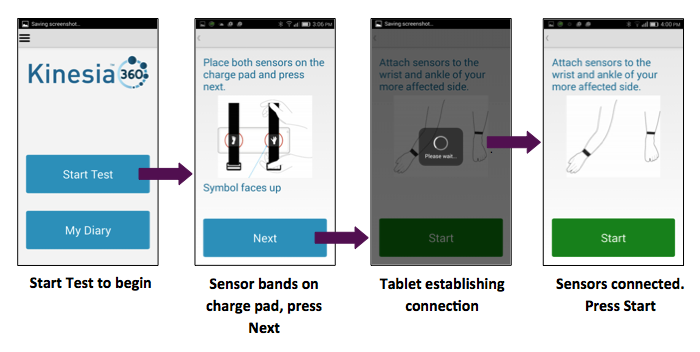
\includegraphics[width=0.75\textwidth]{img/kinesia360.png}
        \caption{Funcionamiento del dispositivo Kinesia 360 \cite{website:glneurotech}.}
        \label{fig:kinesia360}
    \end{figure}
    
    \item \textbf{Personalized Kinetigraph, PKG:} se trata de un biosensor de muñeca (reloj PKG) como se muestra en la Figura \ref{fig:PKG}, diseñado para registrar los movimientos continuamente y cuantificar los temblores, la bradicinesia y la discinesia de los pacientes. Se coloca en la muñeca del lado del cuerpo más afectado. 

    El sistema se basa en el análisis de las señales que provienen de un acelerómetro triaxial colocado en el reloj PKG. Las señales se filtran incluyendo frecuencias entre 0.2 Hz a 4 Hz para obtener dos índices, la aceleración máxima  y el tiempo sin movimiento. Estos valores se corresponden con la bradicinesia y la discinesia, y son registrados cada dos minutos desde el momento en que se coloca el dispositivo hasta que se retira.

    El algoritmo reconoce la bradicinesia como la cantidad de movimientos disminuida que, en comparación con los movimientos normales, se realizan con menor aceleración y amplitud, y con intervalos más largos entre movimientos. Por otra parte, la discinesia se reconoce como la presencia de movimientos con valores de aceleración y amplitud normales pero con periodos cortos sin movimiento
    \cite{griffiths2012automated, website:pkgcare,  santiago2019qualitative}.

    \begin{figure}[ht]
        \centering
        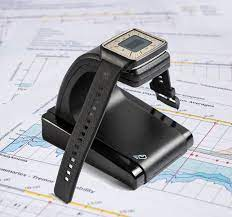
\includegraphics[width=0.35\textwidth]{img/PKG.jpg}
        \caption{Dispositivo Personalized Kinetigraph,PKG \cite{website:pkgcare}.}
        \label{fig:PKG}
    \end{figure}
    
    
    \item \textbf{PD Monitor:} se trata de un sistema de monitorización domiciliaria no invasivo (Figura \ref{fig:PDMonitor}). Está compuesto por cinco dispositivos portátiles de monitoreo para caracterizar todos los síntomas motores de un paciente que provienen de cualquier parte del cuerpo, una aplicación móvil que registra información referida a la medicación, evaluación de síntomas motores y una herramienta que muestra de forma gráfica la información. Emplea un algoritmo basado en técnicas de maching learning.

    Cada uno de los dispositivos de monitoreo presenta un sensor IMU de 9 grados (acelerómetro, giroscopio y magnetómetro) con una frecuencia de muestreo de 59,5 Hz. A través de unos accesorios se fijan al cuerpo del paciente. Los datos recogidos por los dispositivos se transfieren al PDMonitor Smartbox y, posteriormente a la Nube estando disponibles para los médicos.
    La confguración habitual consiste en colocar dos sensores en las piernas, dos en las muñecas y uno en el torso aunque se puede emplear una configuración de dos o tres sensores (pierna, muñeca y torso). De esta manera, no es necesario seleccionar la parte del cuerpo más afectada. 
    
    El sistema se basa en el análisis de las señales del acelerómetro y del giroscopio y se calculan unas determinadas medidas para identificar la posición exacta de cada sensor, así como para discriminar el lado izquierdo o derecho \cite{kostikis2020body}.

    \begin{figure}[ht]
        \centering
        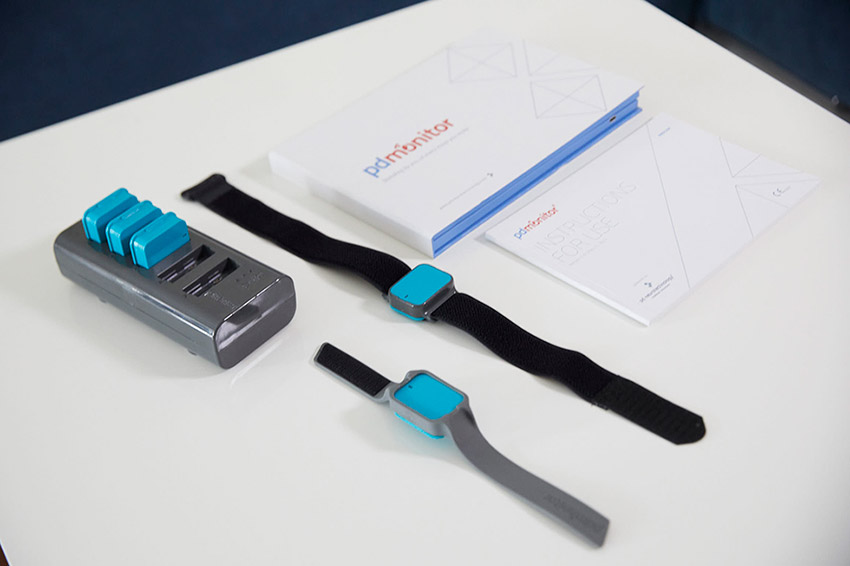
\includegraphics[width=0.4\textwidth]{img/PDMonitor.jpg}
        \caption{Componentes del dispositivo PD Monitor \cite{website:pdneurotechnology}.}
        \label{fig:PDMonitor}
    \end{figure}

    \item \textbf{Sistema REMPARK}: El proyecto REMPARK (\textit{Personal Health Device for the Remote and Autonomous Management of Parkinson's Disease}) tiene por objetivo es desarrollar un sistema de monitorización portátil para identificar el estado motor en tiempo real y evaluar el estado ON/OFF/Discinesia a través de la aplicación de métodos de Inteligencia Artificial.

    Consiste en un cinturon que incluye un acelerómetro triaxial que mide magnitudes de aceleración de -6G a +6G (1G = 9.81 m/s2) con una frecuencia de muestreo de 200 Hz, y las señales obtenidas son analizadas en tiempo real por un microcontrolador. Se emplean dos algoritmos que analizan la marcha, la discinesia y un tercer algoritmo que combina la información de ambos para estimar el estado motor. Los resultados obtenidos se envían por Bluetooth a un teléfono inteligente y después se almacenan en un servidor \cite{bayes2018holter, cabestany2013rempark}.

    La señal del acelerómetro se definió como la suma de los tres ejes de potencia espectral en los rangos [0,1,3] Hz y [0,1,10] Hz en ventanas de 3,2 segundos (128 muestras a 40 Hz) para detectar periodos de marcha. Estas características fueron seleccionadas mediante el algoritmo de selección de características ReliefF y se emplearon como parámetros de entrada para una máquina de vectores de soporte (SVM\footnote{Algoritmo de aprendizaje supervisado empleado en problemas de clasificación y regresión.}). 

    Por otra parte, cuando el paciente presenta discinesia  el espectro de potencia de las frecuencias más bajas aumenta. Se consideró el rango del espectro de potencia de la banda de frecuencias de 1 a 4 Hz para detectar discinesia siempre que las frecuencias más altas (8 a 20 Hz) no presenten un espectro de potencia alto que representan actividades como caminar o subir escaleras \cite{perez2016dopaminergic}.
    
    
    \item \textbf{STAT-ON}: como se puede observar en la Figura \ref{fig:staton}, es un dispositivo portátil que incluye un sensor y se coloca en un cinturón alrededor del paciente permitiendo registrar el estado motor de los pacientes  como bradicinesia, discinesia, fluctuaciones ON/OFF que aparecen en el Parkinson avanzado o caídas entre otros. 

    Internamente, el sistema se compone de dos nano-acelerómetros triaxiales ultrabajos, dos microcontroladores y un sistema Bluetooth de baja energía (BLE). nRF51822 es el microcontrolador principal, maneja los procesos internos e incorpora el sistema BLE. El segundo microcontrolador es el  STM32F415, encargado de operar modelos matemáticos complejos como los clasificadores SVM (\textit{Support Vector Machines}) y calcular las señales proporcionadas por el acelerómetro principal.

    El sistema emplea varios algoritmos para detectar bradicinesia, discinesia y estados ON/OFF. Además, se incorporó el algoritmo FoG (\textit{Freezing of Gait}) que se basa en un enfoque de aprendizaje automático basado en SVM. El objetivo del conjunto algorítmico es identificar y registrar los estados ON y OFF que dependen de un umbral \textit{Beta} obtenido a partir del clasificador SVM y de la detección de los síntomas de discinesia inducidos por levodopa.  
    
    El profesional sanitario configurará el dispositivo únicamente con tres parámetros cruciales para los algoritmos de estimación de la marcha y bradicinesia. Su empleo está destinado  para entornos domésticos,  durante la realización de actividades de la vida diaria. Los resultados obtenidos se muestran de forma gráfica en una aplicación móvil
    \cite{rodriguez2022new}.

    \begin{figure}[ht]
        \centering
        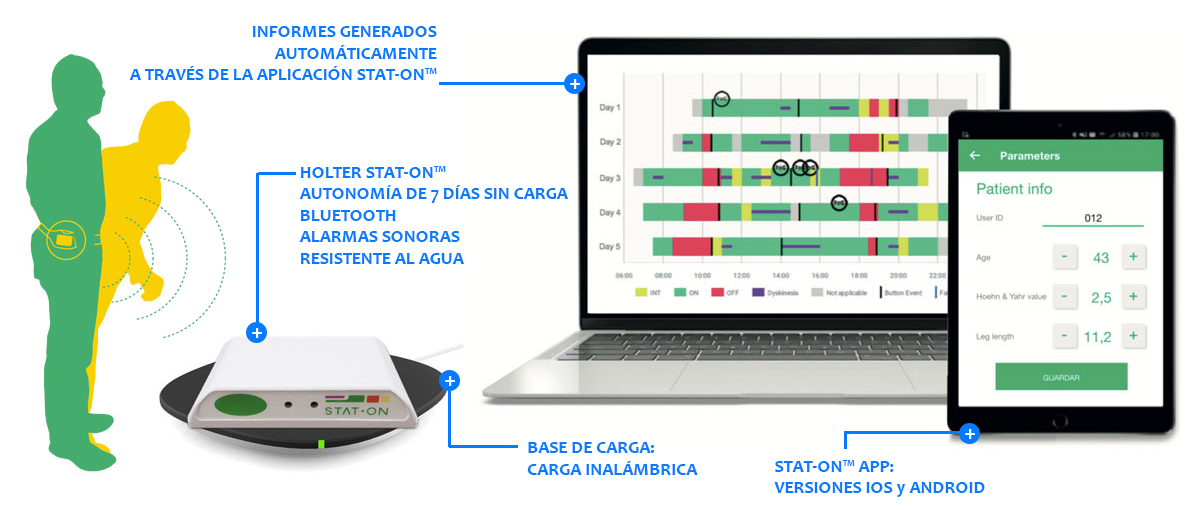
\includegraphics[width=0.7\textwidth]{img/staton-holter.png}
        \caption{Dispositivo STAT-ON \cite{rodriguez2022new}.}
        \label{fig:staton}
    \end{figure}
\end{enumerate}

Por otra parte, los avances tecnológicos permiten el continuo desarrollo de nuevos dispositivos dirigidos a mejorar la adquisición e interpretación de señales con el fin de caracterizar los síntomas motores y analizar la evolución de dichos pacientes. A continuación, se muestran algunos ejemplos:

\begin{enumerate}
    \item Se ha diseñado un sistema portable que obtiene señales eléctricas de la actividad muscular (EMG) de forma simultánea e inalámbrica a partir de las medidas extrínsecas de los síntomas motores parkinsonianos, aceleración, par y velocidad de golpeteo.  Estas medidas se han obtenido empleando un acelerómetro, un dinamómetro y una computadora que administra una prueba de toque con el dedo, respectivamente. 

    En particular, la aceleración está asociada con la potencia espectral EMG en el ancho de banda característica del temblor parkinsoniano y los temblores son detectados a partir de la densidad espectral de potencia (\textit{power spectral density o PSD}) de la señal EMG. El área de la PSD en el rango de 3-6 Hz se utilizó como medida del grado de temblor. Además, para determinar la medida extrínseca de rigidez se empleó una regresión lineal.
    
    Aunque todavía está en desarrollo, el objetivo es el monitoreo continuo de los principales síntomas parkinsonianos (temblor, rigidez y bradicinesia) en base a medidas obtenidas durante las actividades de la vida diaria y, así ofrecer una información más precisa \cite{askari2010emg}.
    
    \item Asimismo, un estudio desarrolló un dispositivo EMG inalámbrico basándose en el microcontrolador NodeMC. A través de tres electrodos de Ag/AgCl se capturan las señales biopotenciales del músculo que se encuentran en la superficie de la piel y son recibidas por el sensor muscular Myware.
    
    A continuación, la señal será amplificada, filtrada y los datos EMG se enviarán al servidor web a través del módulo Wi-Fi ESP8266. Posteriormente, se mostrarán y procesarán en un gráfico de registro de datos en tiempo real en el servidor web. 
    
    La adquisición de datos se llevo a cabo mediante el algoritmo AJAX, lo que permitía que el gráfico de las señales EMG se detuviera si la pestaña o página está cerrada desde el navegador.
    
    También se puede acceder al programa de sistema de monitoreo a través de un teléfono móvil siempre que esté conectado a la misma red Wi-Fi \cite{fadhlannisa2020design}. 
    
    \item Se ha desarrollado una plataforma mHealth denominada PD Manager para el manejo de pacientes con EP. La monitorización de los síntomas motores se realiza a través de la colocación de sensores en una mueñequera y en un par de plantillas combinado con un teléfono inteligente. 
    
    Tanto la pulsera como el teléfono inteligente ofrecen datos sin procesar de un acelerómetro y giroscopio a una frecuencia de muestreo de 100 H. Dichos datos se emplearon para diseñar métodos de evaluación de los síntomas motores. La muñequera incluye diversos sensores como acelerómetro/giroscopio de 3 ejes, sensor de temperatura, sensores capacitativos y galvánicos de respuesta a la piel. 
    
    Por otra parte, el empleo de plantillas con sensores presenta una gran ventaja, ya que permite medir de forma discreta la distribución de la presión del pie, el ritmo de aceleración, la estabilidad y secuencias de movimiento. Cada plantilla está constituído por 13 sensores de presión capacitativos, sensor de aceleración 3D integrado y un sensor de temperatura.

    Una vez obtenidos los datos, son procesados en el microcontrolador integrado para calcular los parámetros necesarios para evaluar la marcha y el movimiento.

    El Servicio mHealth establece la comunicación y transferencia de datos entre las aplicaciones móviles y la plataforma en la nube a través de Internet cumpliendo protocolos de seguridad \cite{gatsios2020feasibility}.
\end{enumerate}




